\section{项目内容}

\subsection{数据预处理}

    \begin{frame}{数据预处理}
    \begin{block}{}
    \begin{enumerate}
        \item 视频转码
        \item 时间点校正和估计
        \item 视频切割
        \item 行人检测
        \item 人工标注
    \end{enumerate}
    \end{block}
    \begin{figure}
    \centering
    \includegraphics[width=\textwidth]{figures/label}
    \caption{数据预处理的最终结果}
    \label{fig:label}
    \end{figure}
    \end{frame}

    \begin{frame}{行人检测效果}
    \begin{block}{}
    检测视频画面帧中的行人,输出bounding box。
    使用Facebook开源的Detectron工具,其实现了Mask RCNN框架。
    \end{block}
    \begin{figure}
    \centering
    \includegraphics[width=0.3\linewidth]{figures/1-2_5_151.jpg}~
    \includegraphics[width=0.3\linewidth]{figures/3-7_10_394.jpg}\\
    \includegraphics[width=0.3\linewidth]{figures/1-2_5_151_det.jpg}~
    \includegraphics[width=0.3\linewidth]{figures/3-7_10_394_det.jpg}
    \caption{Detectron行人检测结果可视化}
    \label{fig:detectron}
    \end{figure}
    \end{frame}

\subsection{行人重识别论文复现}

    \begin{frame}{行人重识别论文复现结果}
    \begin{block}{}
    训练阶段交叉熵误差(Loss)随着数据集训练批次数(Epoch)变化曲线如图\ref{fig:loss}所示。
    行人重识别,指的是在多个视野不重叠的监控视频中,重新识别那些之前出现过的行人,即把当前行人与之前已标记的人物相对应。
    \end{block}
    \begin{columns}[]
    \centering
    \begin{column}{0.6\textwidth}
        \begin{table}
            \centering
            \begin{tabular}{@{}ccccc@{}}
            \toprule
                    & mAP   & Rank1 & Rank10 \\ \midrule
            论文中显示  & 77.3  & 92.4  & 97.9   \\
            复现结果   & 71.1  & 86.2  & 93.4   \\ \bottomrule
            \end{tabular}
            \caption{Market1501数据集测试结果}
            \label{tab:test}
        \end{table}
    \end{column}
    \begin{column}{0.3\textwidth}
        \begin{figure}[]
            \centering
            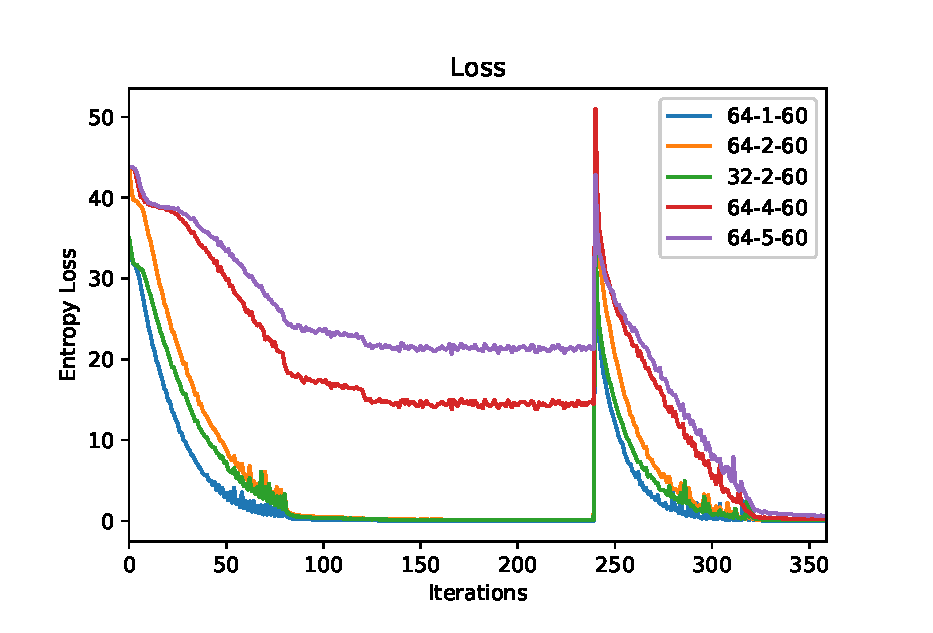
\includegraphics[width=\textwidth]{figures/loss}
            \caption{交叉熵误差随迭代数变化曲线}
            \label{fig:loss}
        \end{figure}
    \end{column}
    \end{columns}
    \end{frame}

    \begin{frame}{测试结果可视化}
        \begin{columns}
            \begin{column}{0.5\textwidth}
                图\ref{fig:testvis}是测试结果的可视化,左边一列是查询图片,每一张查询图片相应的右边一行是从测试库中挑选出来的图片,有红色边框的图片代表该人物标签与相应的查询图片人物标签不一致。
            \end{column}
            \begin{column}{0.5\textwidth}
                \begin{figure}
                \centering
                \includegraphics[width=\textwidth]{figures/vis3}
                \caption{测试结果可视化}
                \label{fig:testvis}
                \end{figure}
            \end{column}
        \end{columns}
    \end{frame}

\subsection{强化学习}

    \begin{frame}{经强化学习后选择的部署方案}
    \begin{block}{}
    使用Q-Learning算法,表\ref{tab:rlresult}为经过强化学习训练后的智能体在应对各种状态时,最有可能采取的行动统计。最优方案下的监控画面如图\ref{fig:rlresult}所示。
    \end{block}
    \begin{columns}
        \begin{column}{0.5\textwidth}
            \begin{table}
                \centering
                \begin{tabular}{@{}ccc@{}}
                \toprule
                方案               & 频次  & 占比      \\ \midrule
                (1, 2, 7, 10, 14) & 190 & 65.97\% \\
                (1, 2, 7, 10, 13) & 78  & 27.08\% \\
                (1, 2, 7, 9, 14)  & 18  & 6.15\%  \\
                (1, 3, 7, 10, 14) & 1   & 0.35\%  \\
                (0, 2, 7, 10, 14) & 1   & 0.35\%  \\ \bottomrule
                \end{tabular}
                \caption{学习后选择的部署方案}
                \label{tab:rlresult}
            \end{table}
        \end{column}
        \begin{column}{0.5\textwidth}
            \begin{figure}
            \centering
            \includegraphics[width=0.3\textwidth]{figures/1-2}
            \includegraphics[width=0.3\textwidth]{figures/1-4}\\
            \includegraphics[width=0.3\textwidth]{figures/2-3}
            \includegraphics[width=0.3\textwidth]{figures/3-2}
            \includegraphics[width=0.3\textwidth]{figures/3-6}
            \caption{最优部署方案}
            \label{fig:rlresult}
            \end{figure}
        \end{column}
    \end{columns}
    \end{frame}

